\clearpage
\section{Archived Robot Recordings and Garage Routes}\label{app:routes}
\begin{center}\small
\begin{tabular}{lrrr}
\toprule
Recording & Minutes & Path (m) & Map points \\
\midrule
roabag2336 & 3.1 & 84.5 & 178,179 \\
rosbag0521\_2 & 4.0 & 108.8 & 199,568 \\
rosbag2245 & 9.8 & 316.2 & 565,791 \\
rosbag2\_20260415\_174148 & 18.9 & 556.9 & 2,148,498 \\
20260414\_4 & 24.3 & 838.4 & 2,778,455 \\
rosbag2\_20260415\_162852 & 27.4 & 834.9 & 3,063,285 \\
\bottomrule
\end{tabular}

\captionof{table}{Original six-recording inventory. Path lengths are trajectory estimates, not ground truth; map point counts belong to the reviewed geometric-map revision, not the current semantic output.}
\end{center}
Recordings may revisit the same sites. They are not six independent semantic tests. Atlas point colors encode height, with deterministic subsampling and central 99\% XY display extent; each route has its own scale. These reviewed offline-backend coordinates are not mixed with later garage or outdoor semantic-map revisions.
\begin{center}
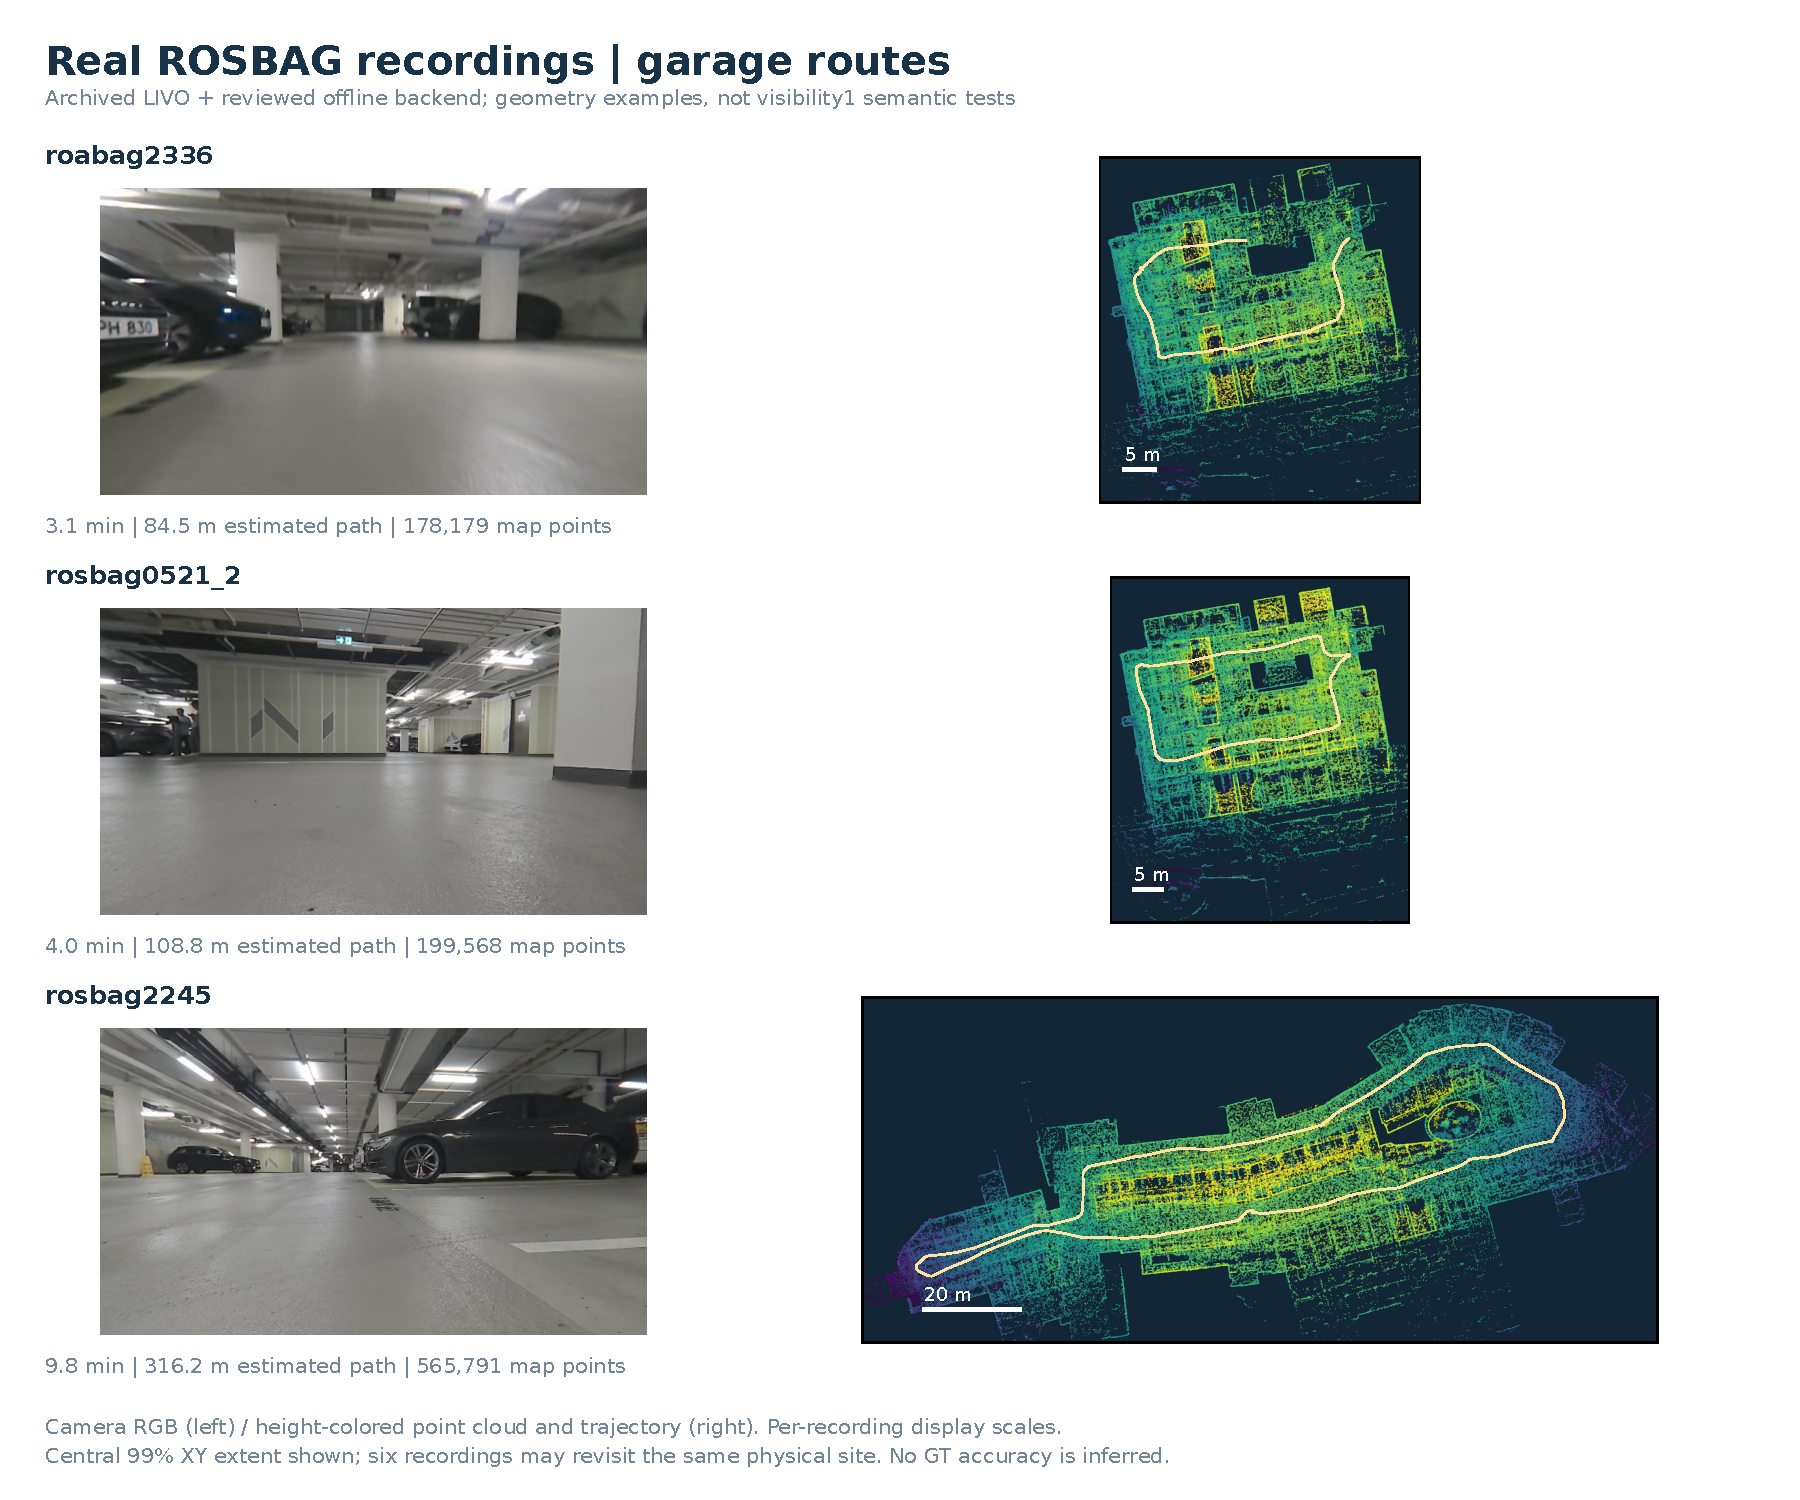
\includegraphics[width=.96\textwidth]{rosbag_routes_1.pdf}
\captionof{figure}{Three actual garage recordings: undistorted camera views, height-colored LiDAR maps and estimated trajectories. These archived sensing results predate the current revision comparison.}
\end{center}
The separate current garage comparison uses the sealed 330-frame semantic branch and the same authorization kernels as the new public assessment. Its results are reported in Appendix~\ref{app:robot}, not inferred from this atlas or its point counts.

\clearpage
\section{Archived Outdoor Routes}
\begin{center}
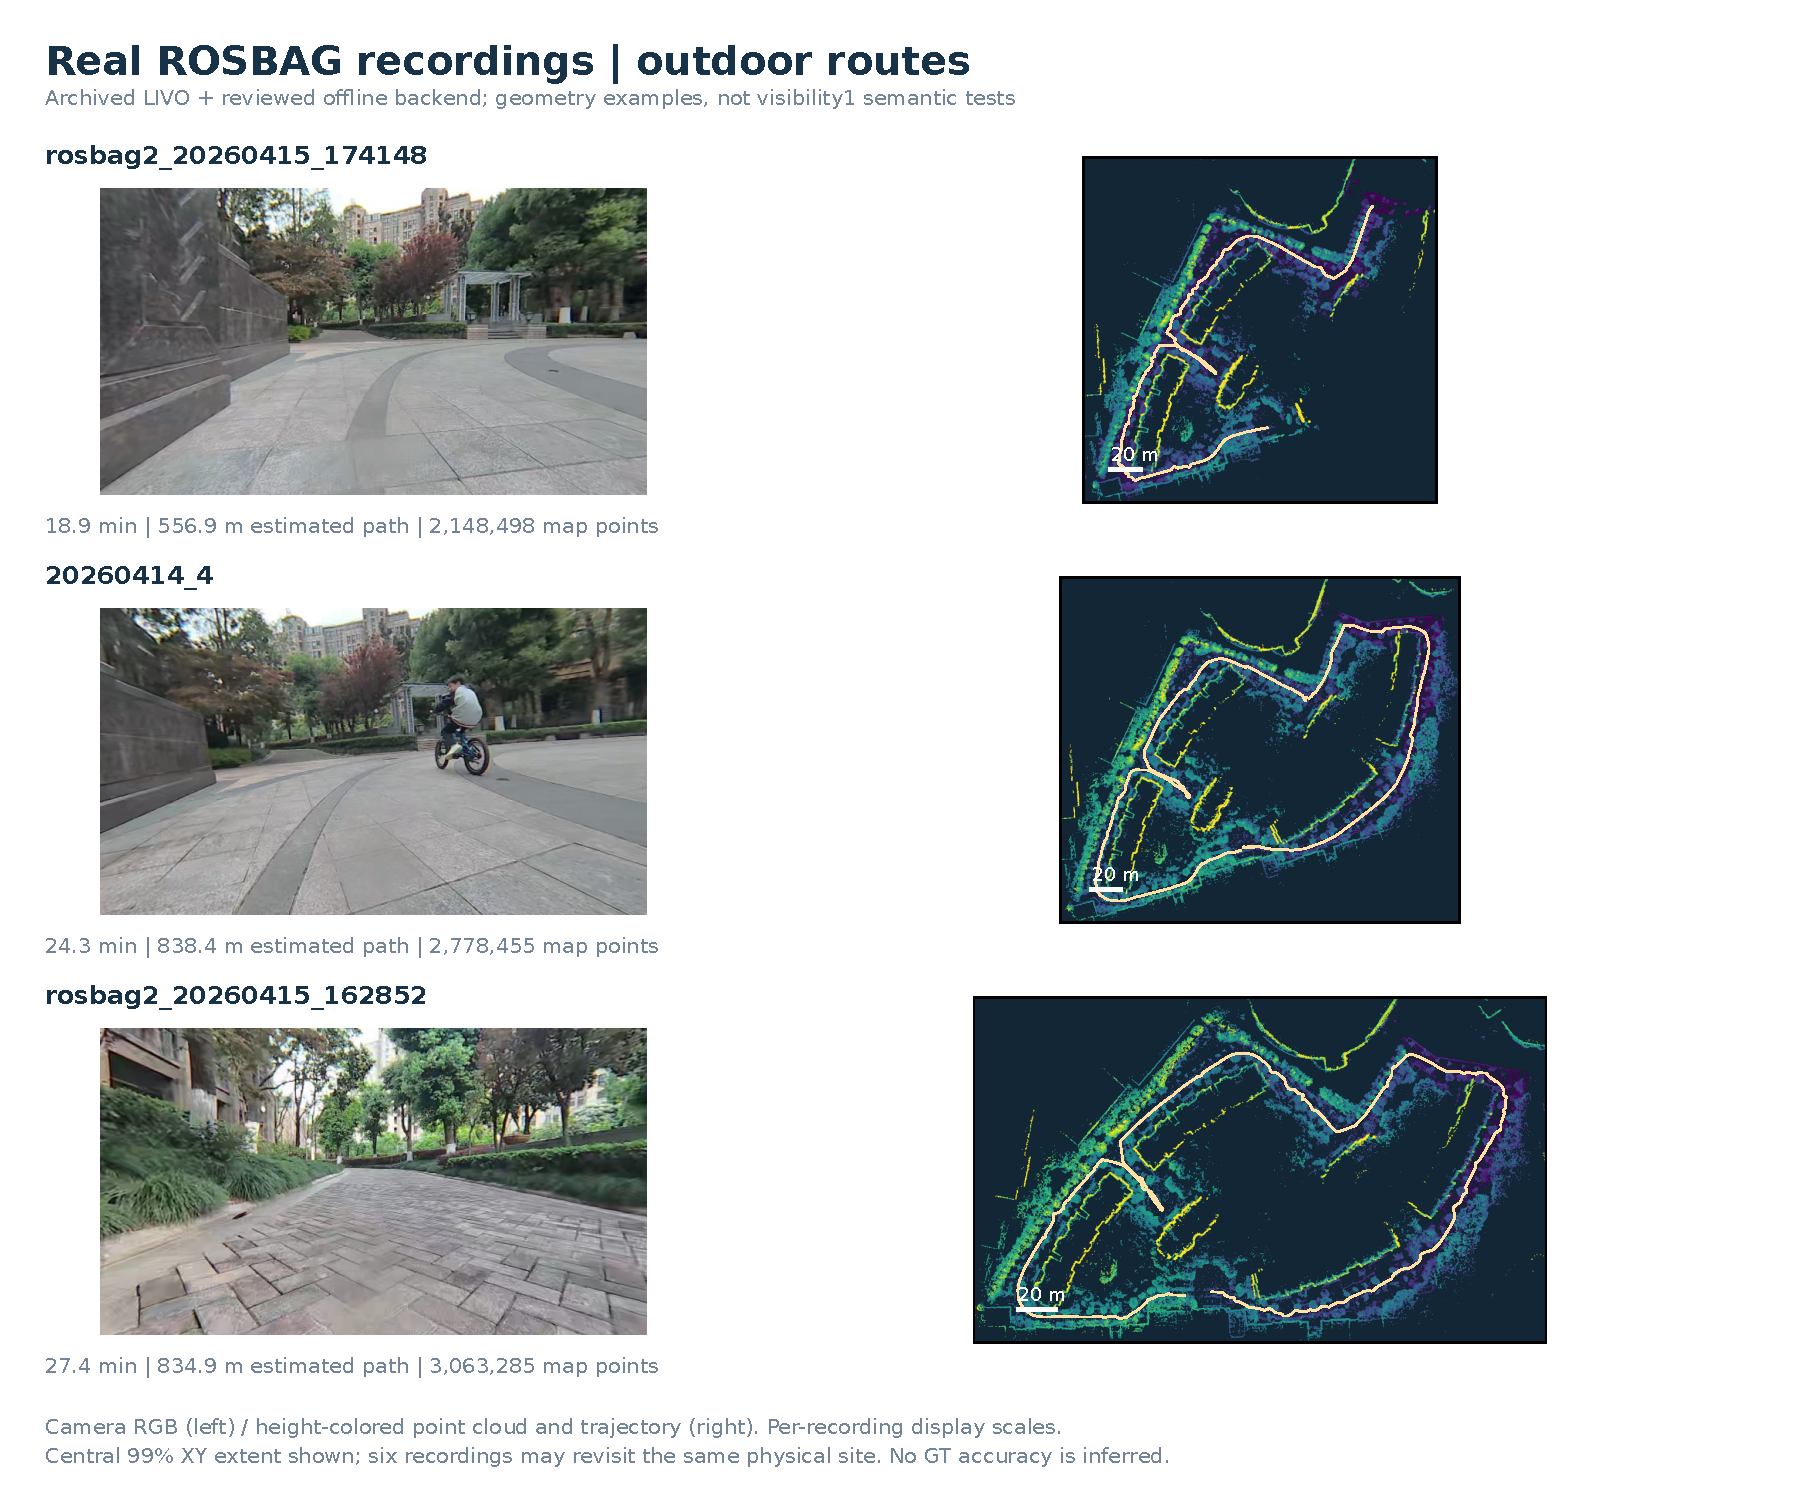
\includegraphics[width=.98\textwidth]{rosbag_routes_2.pdf}
\captionof{figure}{Three actual outdoor recordings, including estimated paths around 835 and 838\,m. Height colors and per-recording scales match the garage atlas conventions. Spatial overlap is possible; neither independent-site generalization nor current-method semantic accuracy follows.}
\end{center}
\subsection{System and map-version provenance}
The outdoor semantic record \texttt{rosbag2\_20260415\_162852} contains 440 keyframes. Grounding DINO tiny produces image detections, followed by measured-depth association. The archived static map retains 19 repeated-observation records (15 plant and four door/entrance candidates). These counts are prediction records, not verified unique physical objects. SegFormer B0 with Cityscapes weights proposes image-level ground support; local geometric checks select measured LiDAR points.

The original garage object-evidence branch uses its own \texttt{omni\_odom} coordinates and retained 40 records (34 cars, five doors, one pipe) under SAM2.1/SigLIP/history2. It differs from both the geometric-route atlas and the current 68-ID authorization output. No detections, boxes, masks, or trajectories are transferred between these revisions in this document.

The following pages retain the outdoor landmark and ground examples from their internally consistent original revision. They show useful sensing and evidence interfaces. They are not additional evaluations of either V1 or current \ours{}, and no unannotated semantic-accuracy or real-time claim is attached to them.

\clearpage
\section{Archived Outdoor Landmarks and Measured Bounds}
\begin{center}
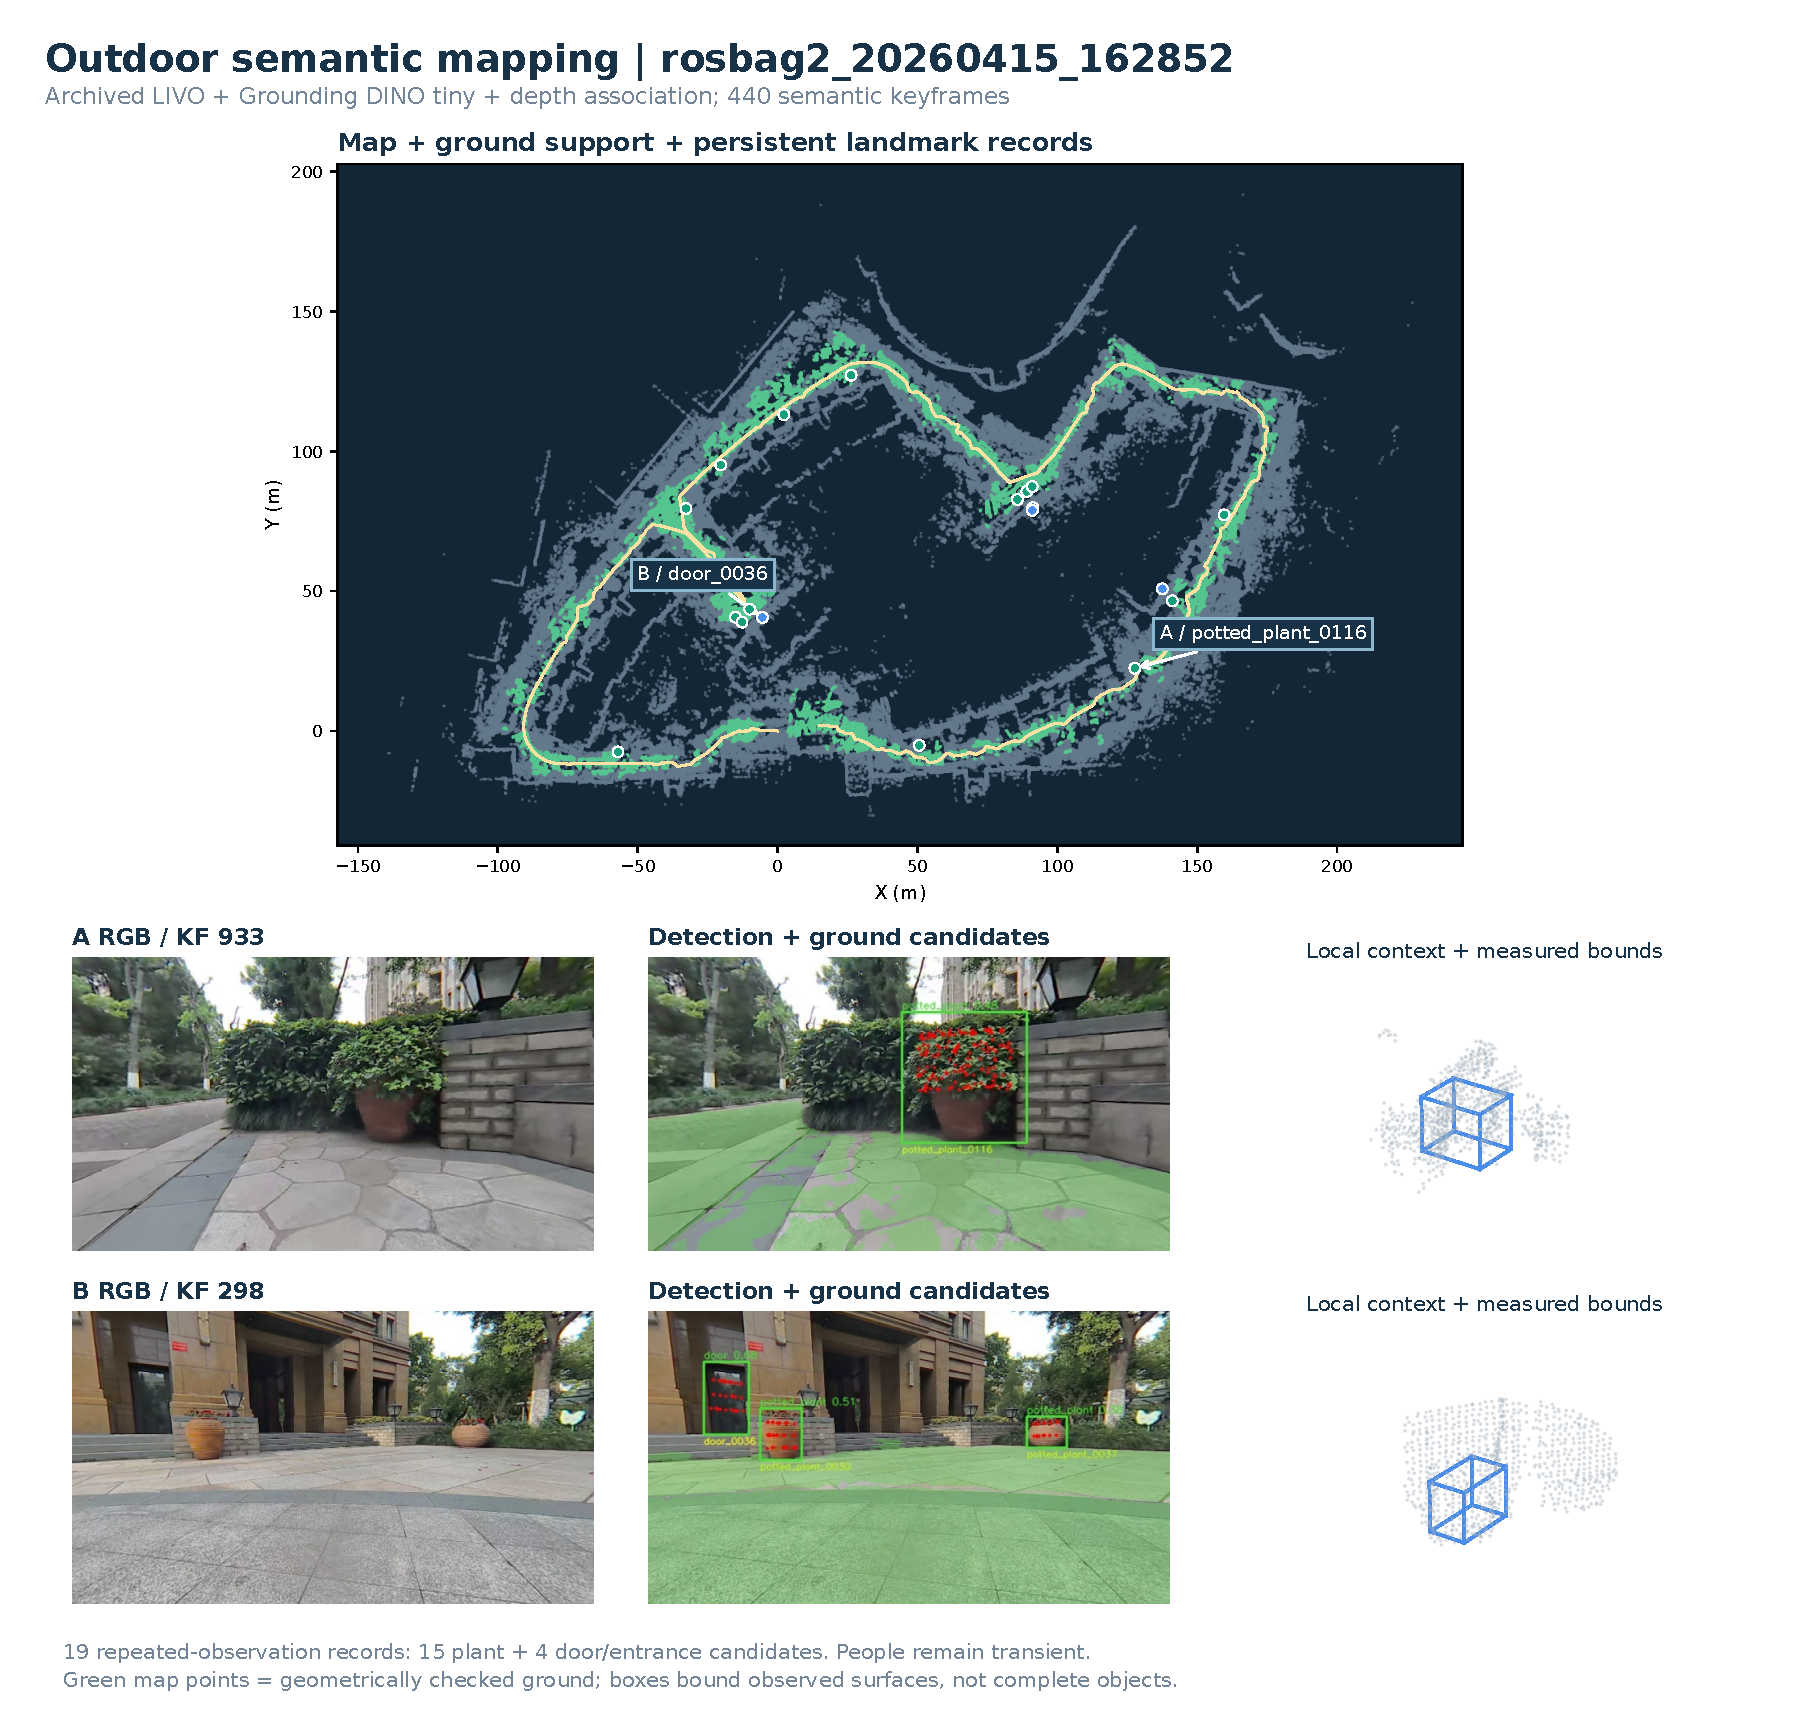
\includegraphics[width=.98\textwidth,height=.78\textheight,keepaspectratio]{rosbag_outdoor_semantics.pdf}
\captionof{figure}{Archived outdoor semantic map, route, checked ground support, and two selected records linked to real images and measured bounds. Gray local points are context, not isolated object geometry. Each record shows its largest observed image box. Categories and boxes are predictions; measured bounds are not independently evaluated 3D detections or full object shapes.}
\end{center}
These images and point clouds were retained without new inference. Coordinates are those of this archived outdoor semantic branch. The figure documents the observation-to-object interface; it does not establish a gain from the current revision module.

\clearpage
\section{Archived Ground and Transient Observations}
\begin{center}
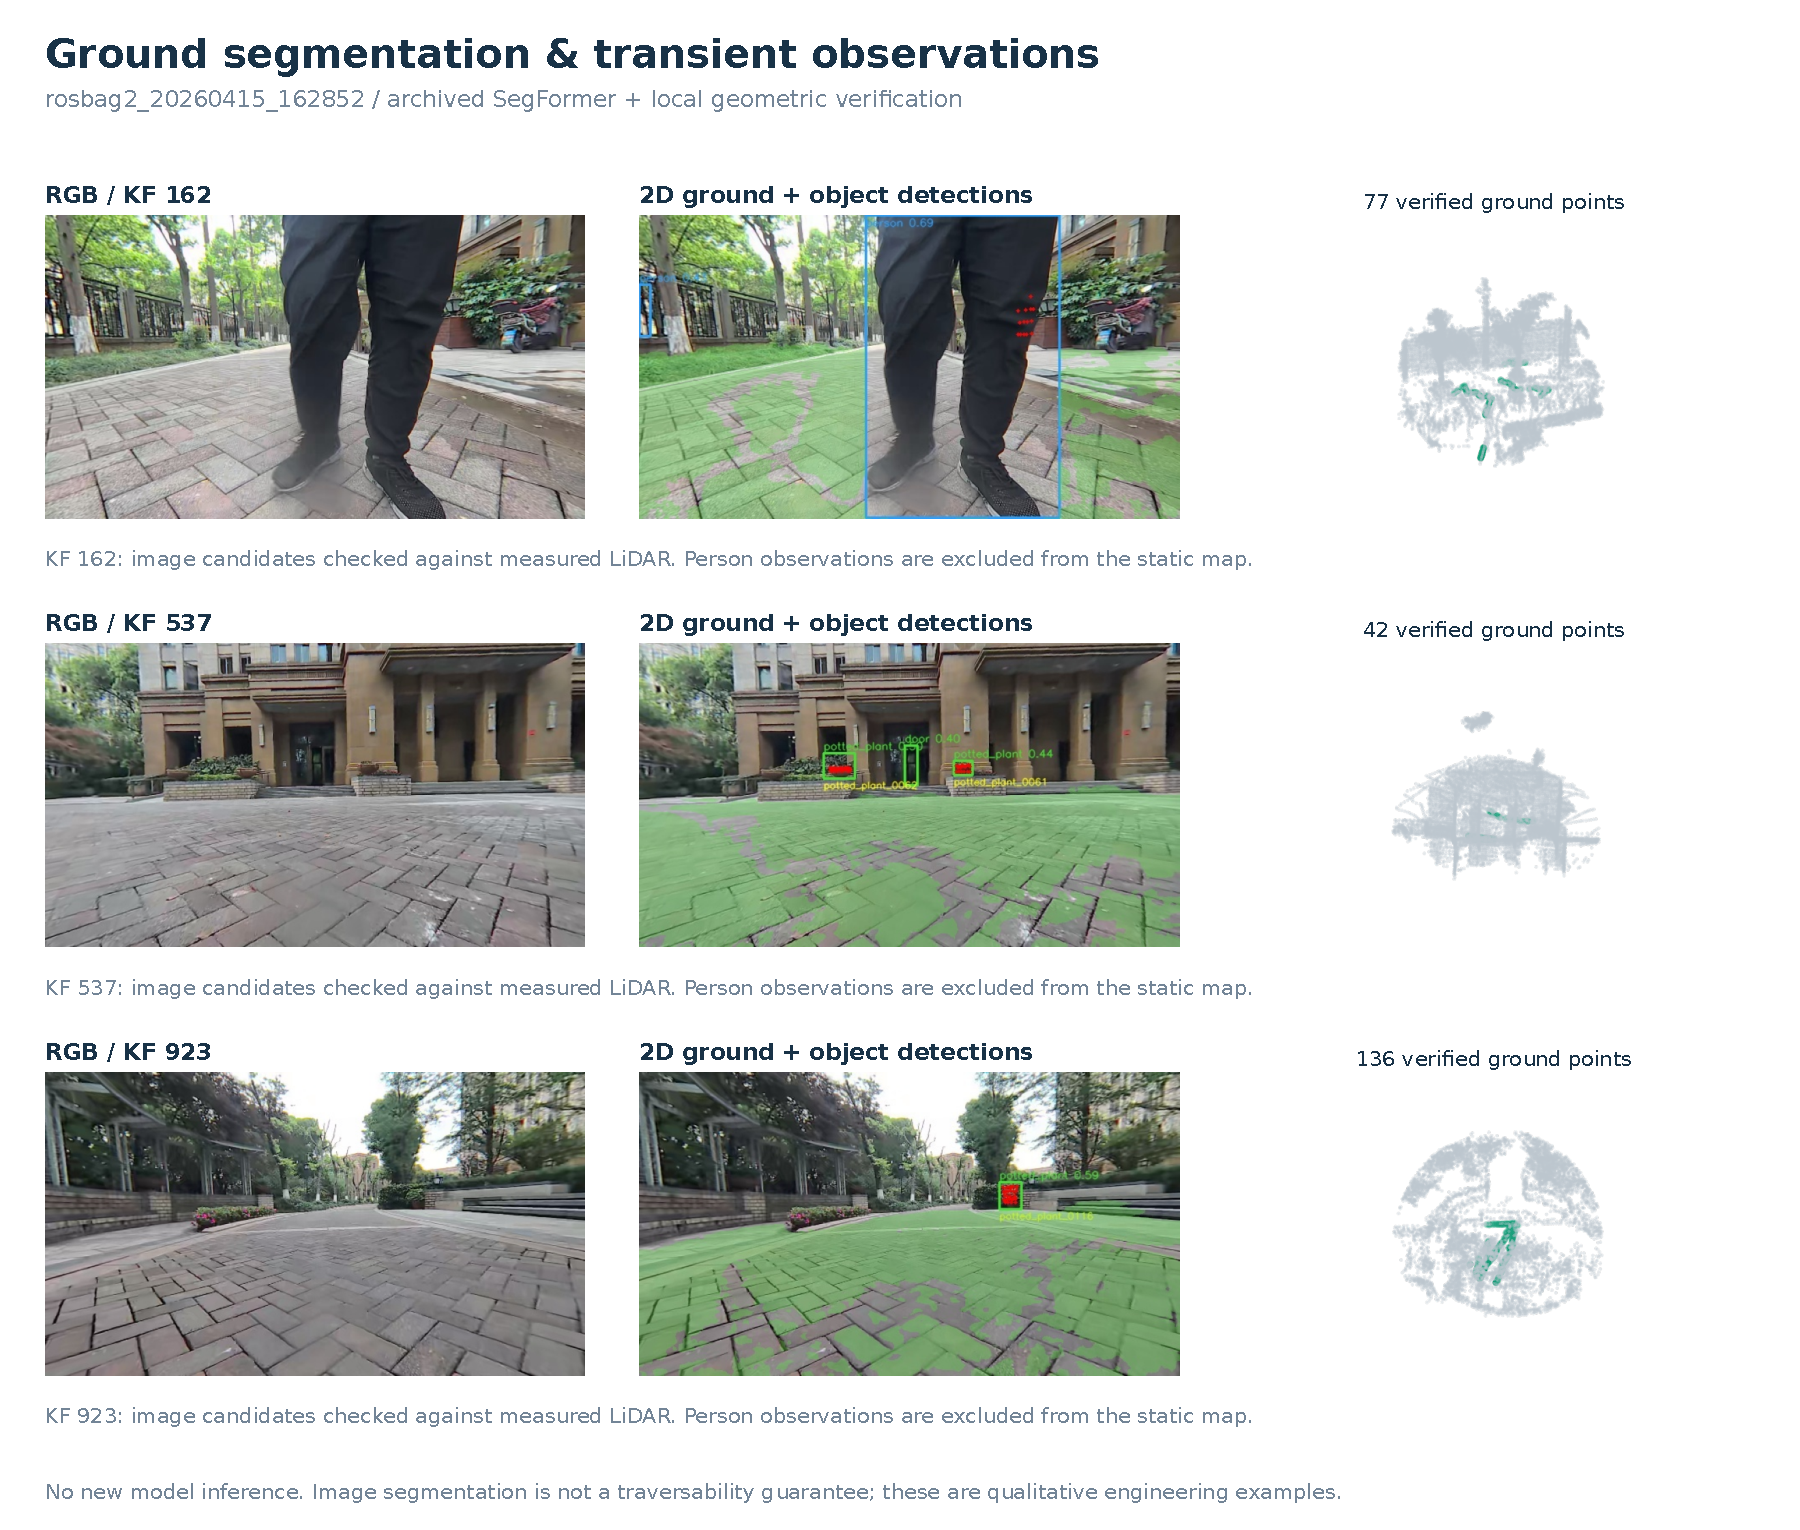
\includegraphics[width=.98\textwidth,height=.78\textheight,keepaspectratio]{rosbag_ground_details.pdf}
\captionof{figure}{Three actual outdoor keyframes: RGB, image-level ground candidates and detections, and geometrically checked LiDAR ground support. Image candidates and accepted 3D points are different outputs. Selected frames have nonempty accepted support; other frames may not. People remain transient observations and are excluded from static landmarks.}
\end{center}
These examples preserve the original scope: qualitative ground/object interfaces rather than a traversability guarantee, a quantitative ground-segmentation benchmark, or a current-method result. The archived maps remain separate from the new KITTI-360 reference domain and the current garage comparison.
